% Title: I see dead authors
% Author: Jakob Voß
%
% This diagram shows several OMR2 features in a relatively small model
\documentclass{article}
\usepackage{tkz-orm}
\usetikzlibrary{positioning}
\begin{document}
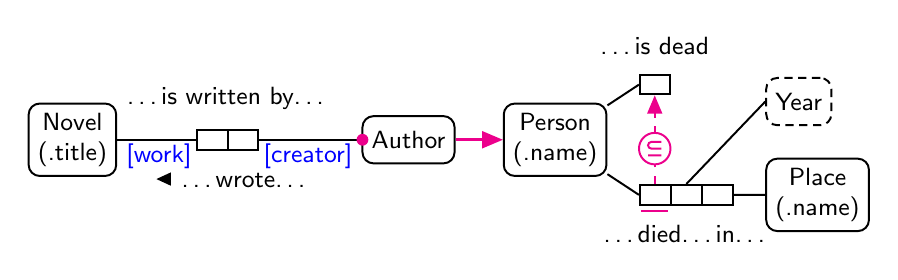
\begin{tikzpicture}[orm]

% entity type (one with reference mode, one without)
\entity (person) {Person\\(.name)};
\entity (author) [left=6mm of person] {Author};

% unary relationship with label
\unary (dead) [right=of person,yshift=7mm,label=\ldots is dead] {};

% binary relationship with labels in both directions
\binary (wrote) [left=13mm of author,
  label=\ldots is written by\ldots,
  label=below:\ormleft{\ldots wrote\ldots}] {};

% role names
\node[role name,anchor=north east] at (wrote.west) {[work]};
\node[role name,anchor=north west] at (wrote.east) {[creator]};
\plays (person) to (dead.west);

% mandatory role constraint
\entity (novel) [left=10mm of wrote] {Novel\\(.title)};
\plays[mandatory] (author) to (wrote);
\plays (wrote) to (novel);

% ternary relationship with uniqueness constraint
\ternary (died) [right=of person,yshift=-7mm,unique=-1,
                 label=below:{\ldots died\ldots in\ldots}] {};
\plays (person) to (died.west)
   (died.east) to +(4mm,0) node[entity,anchor=west] (place) {Place\\(.name)};

% value type
\value (year) [above=of place.north west,anchor=south west] {Year};
\plays (died.north) to (year.west);

% subtyping 
\draw[subtype] (person) to (author);

% subset constraint
\draw[limits to] (died.one north) to (dead.south);
\node[constraint=subset] at ($(died.one north)!0.4!(dead.south)$) {};

\end{tikzpicture}
\end{document}